\documentclass[norsk,a4paper,12pt]{article}
\usepackage[utf8]{inputenc}
\usepackage{physics}   % Matrixes and Dirac-notation
\usepackage{tabularx}  % Tables
\usepackage{booktabs}  % Table rules
\usepackage{graphicx}  % Pictures/figures
\usepackage{listings}  % Source code
\usepackage{color}     % Colors
\usepackage{hyperref}  % Hyperlinks
\usepackage{float}     % Pin figures
\usepackage{titlesec}  % For nice abstract 
\usepackage{tikz}      % For drawing directly in LaTeX
\usetikzlibrary{positioning}

\definecolor{dkgreen}{rgb}{0,0.6,0}
\definecolor{gray}{rgb}{0.5,0.5,0.5}
\definecolor{mauve}{rgb}{0.58,0,0.82}
\definecolor{orange}{RGB}{255,153,0}
\definecolor{lime}{RGB}{173,255,47}
\definecolor{grey}{RGB}{211,211,211}
\definecolor{darkblue}{RGB}{0,0,139}

%Defining source code
\lstset{frame=tb,
  language=c++,
  aboveskip=3mm,
  belowskip=3mm,
  showstringspaces=false,
  columns=flexible,
  basicstyle={\small\ttfamily},
  backgroundcolor=\color{white},
  frame=single,
  numbers=none,
  numberstyle=\tiny\color{gray},
  keywordstyle=\color{dkgreen},
  commentstyle=\color{blue},
  stringstyle=\color{mauve},
  breaklines=true,
  breakatwhitespace=true,
  showspaces=false,
  showtabs=false,
  tabsize=3,
  postbreak=\raisebox{0ex}[0ex][0ex]{\ensuremath{\color{red}\hookrightarrow\space}}
}

\setcounter{secnumdepth}{4}
\titleformat{\paragraph}
{\normalfont\normalsize\bfseries}{\theparagraph}{1em}{}
\titlespacing*{\paragraph}
{0pt}{2.25ex plus 1ex minus .2ex}{1.5ex plus .2ex}


\title{FYS3150 - Computational Physics\\\vspace{2mm} \Large{Project 4}}
\author{\large Even Marius Nordhagen}
\date{\today}
\begin{document}

\maketitle
\begin{abstract}
In this project we use the two dimensional Ising model with periodic boundary conditions to study phase transitions. To estimate the critical temperature of magnetic systems we use Monte Carlo cycles controlled by the Metropolis algorithm. We found the critical temperature to be $T_c'=2.265$, which differs from the exact solution with an error of $\sim4\cdot10^{-3}$. We also compare CPU time required to run the program with and without parallelized processes, and observe the speed-up to be more than two for the parallelized case.
\end{abstract}
The source files and results have been developed in close cooperation with Dorthea Gjestvang and Richard A. Fauli. The former can be found in the link below:
\begin{itemize}
\item \href{https://github.com/richaraf/Comphys_projects/tree/master/Project_4}{Github Repository for the source files used in Project 4$\quad$}\cite{Repository}
\end{itemize}


\section{Introduction}
The aim of this project is to study and simulate phase transitions using the famous square-lattice Ising model, which is a simple model of interacting magnetic spins. The Ising model is named after Ernest Ising, who demonstrated that a phase transition is not possible for a linear chain of two-state spins at finite temperature for one dimension, while the Norwegian physicist Lars Onsager solved the square-lattice version analytically. The model has probably become so popular because it has an easy Hamiltonian in the same time as it's quite intuitive. \cite{Ising}.\par 
In the theory section I will show how one can express some quantities of the model and find their values analytically using periodic boundary conditions for a small lattice, and it will turn out that the analytical method is really comprehensive compared to a numerical solution. In the numerical implementation we use methods to speed up the computations in interaction with the Metropolis algorithm, which is described in the section called method and implementation. First we ran the program for various parameter values, and we compared the numerical solutions to the analytical in benchmarks for several numbers of Monte Carlo cycles. Secondly the absolute error is computed for the same values and displayed in tables, which are found in the result section. The results are finally discussed in the discussion section.

\section{Theory}
\subsection{Ising model}
We are studying the Ising model for a finite number of magnetic moment $L$ in each direction, in total $N=L^D$ spins where $D$ is the number of dimensions. Each magnetic moment will have spin $s=\pm1$, which we often call spin up or spin down and visualize with up- and down arrows. The system will have a initial microstate, where we are able to calculate the energy with the specific formula for the energy in an Ising model without an external magnetic moment
\begin{equation}
E=-J\sum_{<kl>}^Ns_ks_l
\label{eq:Energy}
\end{equation}
which is a double sum where $s_k$ is a spin state and $s_l$ is one of its nearest neighbours. The brackets indicate that we shall only sum over the nearest neighbours, but we are not supposed to calculate the energy for the same interactions twice! This is reasonable because the spin can only exchange energy with the nearest neighbours. $J$ is a positive constant with energy units, and indicates the strength of the interactions (should not be confused with Joule). The magnetization of the microstate is simply given by the sum over all the spins
\begin{equation}
M=\sum_k^N s_k.
\label{eq:Magnetization}
\end{equation}
If the system is at rest we say that it is in steady state, but this is not really probably if we start with a random microstate. Then the system will flip a spin (from up to down or vice versa), and we will have a new microstate with different energy and magnetization than the previous. This can be calculated in the same way as we did for the initial microstate, and we will find a energy difference $\Delta E$. This energy difference determines if the flip is accepted or not, in some cases we need to reset the flip. The indices of the flipped spins are chosen randomly, and when we have been flipping the spin $L\times L$ times (equivalent to the total number of spins in the system), we have done a Monte Carlo cycle. By doing this plenty of times, the system will converge against the steady state, and we get a realistic picture of the behaviour of the system. If we assume that the flips are uniform distributed in time, we can give the time in number of Monte Carlo cycles (I'll refer to the number of Monte Carlo cycles (time) as $t$ and the total numbers of flips as $C$ in the rest of the report). 

\subsection{Numerical expressions}
There can be useful to calculate the average values of the energy and magnetization when we are studying the behaviour of the system over time. Numerically we can find them by calculating the total energy divided by the time, written mathematically as 
\begin{equation}
\langle E\rangle = \frac{1}{t}\sum_{i=0}^t E_i\quad\text{and}\quad
\langle M\rangle = \frac{1}{t}\sum_{i=0}^t M_i
\end{equation}
where we sum over the microstates. Notice that we are normalizing with respect to the time. We will also need the average values squared
\begin{equation}
\langle E^2\rangle = \frac{1}{t}\sum_{i=0}^t E_i^2\quad\text{and}\quad
\langle M^2\rangle = \frac{1}{t}\sum_{i=0}^t M_i^2,
\end{equation}
and from this we can calculate the numerical heat capacity and the susceptibility for a system using the formulas
\begin{equation}
C_v=\frac{\langle E^2\rangle - \langle E\rangle^2}{k_BT^2}
\label{eq:Heat}
\end{equation}
and
\begin{equation}
\chi=\frac{\langle M^2\rangle - \langle M\rangle^2}{k_BT}.
\label{eq:suscept}
\end{equation}
$T$ is the temperature and $k_B$ is Boltzmann's constant. We can also use the expectation values to calculate the variance of a quantity $A$, defined by
\begin{equation}
\sigma_A^2=\langle A^2\rangle-\langle A\rangle^2
\end{equation}
which is a measurement of the spread of the numbers in a dataset. We can use this to calculate the standard deviation (STD), which is the square root of the variance (STD$=\sqrt{\sigma_A^2}=\sigma_A$). If we know the value of the STD, we can find the area where most of the data points are collected. One should keep in mind that there is only a constant which differs the variance of the energy from the heat capacity, and the variance of magnetization from susceptibility. 

\subsection{Periodic Boundary Conditions (PBC)}
In Project 4 we are restricted to a quadratic Ising model in two dimensions, which can be set up as a lattice with $L\times L$ spins: 
\begin{center}
  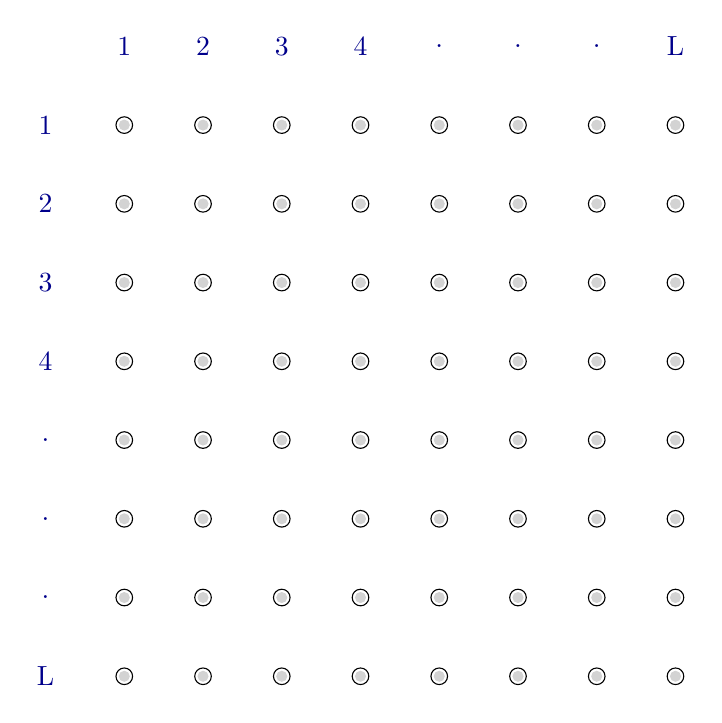
\begin{tikzpicture}
    % labels
    \path[darkblue] (0,8) node{1} (-1,0) node{L};
    \path[darkblue] (1,8) node{2} (-1,1) node{.};
    \path[darkblue] (2,8) node{3} (-1,2) node{.};
    \path[darkblue] (3,8) node{4} (-1,3) node{.};
    \path[darkblue] (4,8) node{.} (-1,4) node{4};
    \path[darkblue] (5,8) node{.} (-1,5) node{3};
    \path[darkblue] (6,8) node{.} (-1,6) node{2};
    \path[darkblue] (7,8) node{L} (-1,7) node{1};
    % loop over the lattice points
    \foreach \i in {0,...,7}
      \foreach \j in {0,...,7}{
        \draw (\i,\j) circle(3pt);
        % check if (\i,\j) > (2,2)
        \ifnum \i < 10
          \ifnum \j < 10
            \fill[grey] (\i,\j) circle(2pt);
          \fi
        \fi
      };
  \end{tikzpicture}
\end{center}
Because of the lattice structure the Ising model will generate boundary problems, which can be treated in some different ways. One solution is to treat the system as a periodic lattice where an edge interacts with the edge on the opposite side of the lattice, called periodic boundary conditions (PBC). This means that we need to take care of the spins on the other side of the lattice when we compute the energy of the edge spins. One way to imagine the PBC of the lattice is to turn the lattice into a closed surface formed as a torus where all the spins have four neighbours. 
 
\subsection{Dimensionless variables and scaling}
There is reasonable to scale the variables such that they become dimensionless to make the expressions as general as possible. The most obvious quantity to scale in this project is the energy, which is given in $J$'s. By dividing by $J$ on both sides of the energy expression, we get dimensionless energy. We are going to deal with temperature, and we want this to be dimensionless as well. This is done by specifying the quantity $T'=k_BT/J=1/J\beta$ (where $\beta=1/k_BT$) which is going to be used regularly. Another property of scaling that is really useful is our case, is the fact that we can scale with respect to small constants which may lead to truncation error when doing numerical calculations. For instance the heat capacity is normally expressed in the same units as $k_B$, but with our specification of the temperature, we can use the units $[C_v/k_B]=1/(T')^2$.  The temperature is the only unknown variable, so there is reasonable to express the quantities as functions of $T'$. The susceptibility has dimension energy inverse, so this quantity can simply be scaled to dimensionless units with multiplying with $J$: $[\chi\cdot J]=1/T'$. The magnetization is already dimensionless.\par\vspace{5mm}

\subsection{Analytical expressions and values}
\subsubsection{Microstates and macrostates of L=2}
We can calculate the energies and magnetizations of all the microstates of a $L\times L$ lattice using Formula (\ref{eq:Energy}) and (\ref{eq:Magnetization}). For a $2\times2$ lattice with PBC the result can be found in Table (\ref{tab:analytical}).  
\begin{table}[H]
\centering
\caption{Average energy and magnetization for the two-dimensional Ising model with $L=2$ spins with PBC.}
\label{tab:analytical} 
\begin{tabularx}{\textwidth}{XlrrrX}
\toprule
Number of spins up & Degeneracy & Energy, $E/J$  & Magnetization, $M$ \\
\midrule
0   & 1  & -8 & -4    \\
1	& 4  & 0  & -2    \\
2   & 2  & 8  & 0     \\
2   & 4  & 0  & 0     \\
3   & 4  & 0  & 2     \\
4   & 1  & -8 & 4     \\
\bottomrule
\end{tabularx}
\end{table}
An interesting aspect with the results is that we have an energy doublet for two spins pointing up. How can it be right that the same number of spins up can give different energies? If we take a look at the possible microstates with two spins pointing up, we observe two different symmetries, represented below:
\begin{equation}
\mqty{\downarrow&\uparrow\\ \uparrow&\downarrow}\quad\text{and}\quad
\mqty{\downarrow&\downarrow\\ \uparrow&\uparrow}.
\end{equation}
If we again look at the energy formula given above, we can see that the microstates with symmetry similar the one on the right hand side will have energy $0$ because the energies cancel. For the symmetry on the left hand side the energy will be $-8$.

\subsubsection{Analytical expressions}
For small systems an expectation value of a quantity $A$ can easily be found analytically by a formula widely used in statistical physics
\begin{equation}
\langle A\rangle = \frac{1}{Z}\sum_{i=1}^{2^N}A_ie^{-E_i\beta}
\end{equation}
where $Z$ is the partition function
\begin{equation}
Z=\sum_{i=1}^{2^N}e^{-E_i\beta}
\end{equation}
which is dimensionless and acts as a normalizing constant (in the same way as $t$ in the numerical expressions). The formula states that we need to sum over the energies for all microstates (there exists $2^N$ microstates for a $N=L\times L$ system) and normalizing using $Z$. When $L=2$, we will have 16 possible microstates with the macrostates (degeneracies) listed in Table (\ref{tab:analytical}). By inserting the possible energies into the partition function, we obtain
\begin{equation}
Z=2(e^{-8J\beta}+e^{8J\beta}+6)=4(\cosh(8J\beta)+3)
\end{equation}
where we have used that $2\cosh(x)=e^x+e^{-x}$. We are now able to express the expectation values as function of $T'$, and I will begin with the average energy
\begin{equation}
\langle E(T')\rangle/J = \frac{8e^{-8/T'}-8e^{8/T'}}{e^{-8/T'}+e^{8/T'}+6}= -\frac{8\sinh(8/T')}{\cosh(8/T')+3}
\end{equation}
where the hyperbolic function $2\sinh(x)=e^x-e^{-x}$ is used. The average magnetization $\langle M\rangle$ simply depends on the number of spins up (the orientation doesn't matter) like in the numerical formula, and is equal to 0 because the probability measuring a positive magnetization is equal to the probability measuring a negative magnetization. The same formulas can in the principle be used to express the average values squared, for example when we want to express $\langle E^2\rangle$ we just insert $E^2$ instead of $A$:
\begin{equation}
\langle E^2(T')\rangle/J^2=64\frac{e^{8/T'}+e^{-8/T'}}{e^{8/T'}+e^{-8/T'}+3}=\frac{64\cosh(8/T')}{\cosh(8/T')+3}
\end{equation}
\begin{equation}
\langle M^2(T')\rangle=\frac{8(e^{8/T'}+1)}{\cosh(8/T')+3}.
\end{equation}
Since the average magnetization is equal to 0, there will be more useful to study the average absolute magnetization
\begin{equation}
\langle|M(T')|\rangle=\frac{4(e^{8/T'}+2)}{\cosh(8/T')+6}
\end{equation}
and furthermore we can find analytical expressions for the heat capacity and susceptibility as functions of the temperature using Formula (\ref{eq:Heat}) and (\ref{eq:suscept}):
\begin{equation}
C_v/k_B(T')=\frac{64}{(T')^2}\bigg(\frac{1+3\cosh(8/T')}{(\cosh(8/T')+4)^2}\bigg)
\end{equation}
where the relation $\sinh^2x+\cosh^2x=1$ is central. The susceptibility is easy to calculate since the average magnetization is equal to zero.
\begin{equation}
\chi\cdot J(T')=\frac{1}{T'}\langle M^2\rangle=\frac{1}{T'}\frac{8(e^{8/T'}+1)}{\cosh(8/T')+3}
\end{equation}

Notice: We could have been calculating the average energy and the heat capacity in simpler ways known from thermal physics, but this is not as general and robust as the method used above where we can calculate all the expectation values with the same basic formula, even though they are more comprehensive to calculate. \par\vspace{5mm}

In all the expressions above we are dividing on $T'$, so by far the easiest temperature we can work with analytically is $T'=1.0$. By inserting this value into the analytical expressions for average energy, average energy squared, heat capacity, average absolute magnetization, average magnetization squared, and susceptibility, we get the results in Table (\ref{tab:analyticalvalues}).
\begin{table}[H]
\centering
\caption{The values of the average energy, average squared energy, heat capacity, average squared magnetization, average absolute magnetization and susceptibility for the two-dimensional Ising model with $2\times2$ spins using PBC and where $T'=1.0$.}
\label{tab:analyticalvalues} 
\begin{tabularx}{\textwidth}{lXcr}
&&\\
\toprule
Variable & Symbol & Value\\
\midrule
Average energy & $\langle E\rangle/J$ & -7.98393\\ 
Average squared energy & $\langle E^2\rangle/J^2$ & 63.8714\\ 
Heat capacity & $C_v/k_B$  & 0.128329\\
\midrule
Average absolute magnetization & $\langle |M|\rangle$ & 3.99464\\
Average squared magnetization & $\langle M^2\rangle$ & 15.9732\\
Susceptibility & $\chi\cdot J$ & 15.9732\\
\bottomrule
\end{tabularx}
\end{table}

The analytical values can be stated with good precision because the only uncertainly is the precision of the temperature, so I have included 5 significant digits. As we can see the average squared energy ($\langle E^2\rangle$) is close to the average energy squared ($\langle E\rangle^2$), but not exact. The energy variance is the difference between these quantities. Another thing that is worth to notice is that the values of the average squared magnetization and the susceptibility are equal, which is only the case when $T'=1.0$. The same apply for the heat capacity and the energy variance, and the reason to this is about scaling.

\subsection{Phase transformations and critical temperature}
If a magnetic system goes from a magnetic phase to a phase with zero magnetization, we say that the system has undergone a phase transition. The temperature where this phase transition occurs is the critical temperature of the system, which scales as
\begin{equation}
 T_C(L)-T_C(L=\infty) = aL^{-1/\nu},
 \label{eq:tc}
\end{equation}
with  $a$ a constant. After the phase transition the susceptibility will decrease for increasing temperature, so the critical temperature of the Ising model can be found where the susceptibility is maximal. Similarly we can find the critical temperature where the heat capacity is maximal, so there exists several ways to measure the critical temperature. The value of the constant $a$ can be found by using the critical temperature of at least two different systems (for two different L-values):
\begin{equation*}
\Big(T_C(L_1)-T_C(L=\infty)\Big)-\Big(T_C(L_2)-T_C(L=\infty)\Big)=a(L_1^{-1/\nu}-L_2^{-1/\nu})
\end{equation*}
\begin{equation}
\Rightarrow a=\frac{T_C(L_1)-T_C(L_2)}{L_1^{-1/\nu}-L_2^{-1/\nu}}
\label{eq:a}
\end{equation}
We can now calculate the critical temperature for a system with infinity number of magnetic moment after "measured" the critical temperature for smaller systems, and we will use $\nu=1$.  By reorder Formula (\ref{eq:tc}) we obtain the final formula of the critical temperature.
\begin{equation}
T_c(L=\infty)=T_c(L)-aL^{-1/\nu}.
\label{eq:critical}
\end{equation}
The analytical (exact) value of this temperature was found by Onsager, the same guy mentioned in the introduction, and he shown that the value is exact
\begin{equation}
T_c=\frac{2}{\ln(1+\sqrt{2})}J/k\approx 2.269 J/k.
\end{equation}
\cite{Project_text}. 

\section{Method and implementation} 
We are going to make a program and run it for multiple temperatures and system sizes with a large number of Monte Carlo cycles, something that will require a lot from the processor. This section will be much about how to make a robust program which is fast and can handle a large number of operations. For instance we want to minimize the number of loops, if-statements and especially if-statements in loops. To reduce the CPU time further, there are several methods for optimizing which can be used together or separately.\par
To keep the overview I will demonstrate the ideas with a $3\times3$ lattice, even though this system is far from realistic (in the reality we will have systems with thousands or millions of spins in each direction). 
\begin{center}
  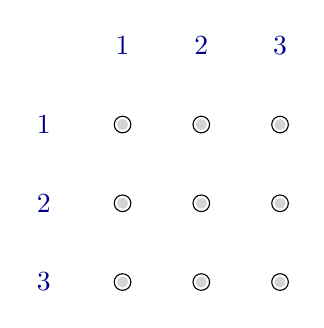
\begin{tikzpicture}
    % labels
    \path[darkblue] (0,3) node{1} (-1,0) node{3};
    \path[darkblue] (1,3) node{2} (-1,1) node{2};
    \path[darkblue] (2,3) node{3} (-1,2) node{1};
    % loop over the lattice points
    \foreach \i in {0,...,2}
      \foreach \j in {0,...,2}{
        \draw (\i,\j) circle(3pt);
        % check if (\i,\j) > (2,2)
        \ifnum \i < 10
          \ifnum \j < 10
            \fill[grey] (\i,\j) circle(2pt);
          \fi
        \fi
      };
  \end{tikzpicture}
\end{center}
Anyway the methods demonstrated in this section are general and can be used on a general lattice, no matter how large it is.

\subsection{Implementation of PBC}
We want to minimize the number of if-statements, so instead of having if-tests that check if a spin is located on the edges, we add the similar edges on the opposite sides. We still only have $N$ spins to take care of (even though the implemented lattice is $L+2\times L+2$), but now they all are located inside the edges and we avoid boundary problems:
\begin{center}
  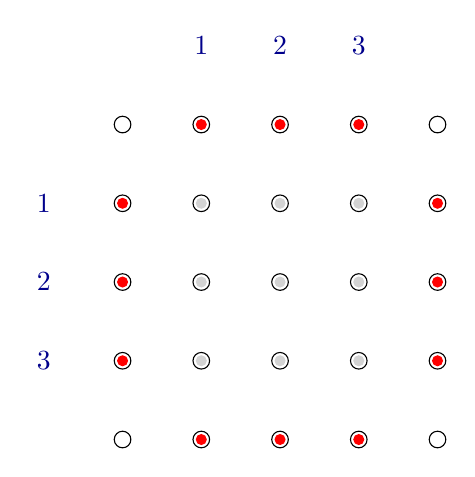
\begin{tikzpicture}
    % labels
    \path[darkblue] (1,5) node{1} (-1,1) node{3};
    \path[darkblue] (2,5) node{2} (-1,2) node{2};
    \path[darkblue] (3,5) node{3} (-1,3) node{1};
    % loop over the lattice points
    \foreach \i in {0,...,4}
      \foreach \j in {0,...,4}{
        \draw (\i,\j) circle(3pt);
        % check if (\i,\j) > (2,2)
        \ifnum \i = 0
          \ifnum \j = 1 
            \fill[red] (\i,\j) circle(2pt);
          \fi
          \ifnum \j = 2 
            \fill[red] (\i,\j) circle(2pt);
          \fi
          \ifnum \j = 3 
            \fill[red] (\i,\j) circle(2pt);
          \fi
        \fi
        \ifnum \i = 1
          \ifnum \j = 1 
            \fill[grey] (\i,\j) circle(2pt);
          \fi
          \ifnum \j = 2 
            \fill[grey] (\i,\j) circle(2pt);
          \fi
          \ifnum \j = 3 
            \fill[grey] (\i,\j) circle(2pt);
          \fi
        \fi
        \ifnum \i = 2
          \ifnum \j = 1 
            \fill[grey] (\i,\j) circle(2pt);
          \fi
          \ifnum \j = 2 
            \fill[grey] (\i,\j) circle(2pt);
          \fi
          \ifnum \j = 3 
            \fill[grey] (\i,\j) circle(2pt);
          \fi
        \fi
        \ifnum \i = 3
          \ifnum \j = 1 
            \fill[grey] (\i,\j) circle(2pt);
          \fi
          \ifnum \j = 2 
            \fill[grey] (\i,\j) circle(2pt);
          \fi
          \ifnum \j = 3 
            \fill[grey] (\i,\j) circle(2pt);
          \fi
        \fi
        \ifnum \i = 4
          \ifnum \j = 1 
            \fill[red] (\i,\j) circle(2pt);
          \fi
          \ifnum \j = 2 
            \fill[red] (\i,\j) circle(2pt);
          \fi
          \ifnum \j = 3 
            \fill[red] (\i,\j) circle(2pt);
          \fi
        \fi
        \ifnum \j = 0
          \ifnum \i = 1 
            \fill[red] (\i,\j) circle(2pt);
          \fi
          \ifnum \i = 2 
            \fill[red] (\i,\j) circle(2pt);
          \fi
          \ifnum \i = 3 
            \fill[red] (\i,\j) circle(2pt);
          \fi
        \fi
        \ifnum \j = 4
          \ifnum \i = 1 
            \fill[red] (\i,\j) circle(2pt);
          \fi
          \ifnum \i = 2 
            \fill[red] (\i,\j) circle(2pt);
          \fi
          \ifnum \i = 3 
            \fill[red] (\i,\j) circle(2pt);
          \fi
        \fi
      };
  \end{tikzpicture}
\end{center}

We can implement the lattice with PBC numerical by a code similar to the pseudo code below.
\begin{lstlisting}
R = matrix(L+2, L+2)

//Fill matrix randomly
for(i = [1,L+1]):
    for(j = [1,L+1]):
        x = integer(rand(0,1))  // x is 1 or 0 
        if(x = 1):
            R(i,j) = 1
        else:
            R(i,j) = -1

//Give Periodic Boundary Conditions
for(i = [0,L]):
    for(j = [0,L]):
        R(0,j+1) = R(L, j+1)
        R(i+1,0) = R(i+1, L)
        R(L+1,j+1) = R(1, j+1)
        R(i+1,L+1) = R(i+1,1)
\end{lstlisting}
To fill the matrix with random spins we need a random number generator (RNG) which is fast, got a long period and has uniform distributed random numbers. We decided to use the built-in RNG in C++, which is pretty fast, but generates just $2^{32}-1\approx5\cdot10^9$ different numbers (this is the period). 

\subsection{Computing energy and magnetization efficiently}
We wish to run the program for a large number of Monte Carlo cycles, and since we need to calculate the energy and magnetization every time, we need to do this efficiently. In the theory section we saw that we can find the energy of a microstate by summing the energy between all neighbours without computing the same interaction energy twice (see Equation (\ref{eq:Energy})). This is easy to avoid when we are calculating the energies analytically, but how do we do that numerically for a general lattice? \par

The clue is to find a way to do the same operation on all the spins (no matter where the spin is located in the lattice), which is possible because of the implementation of the PBC. The idea is to say that all the spins only are exchanging energy with the spin above and on the right hand side, like shown below (we can choose which two neighbours of a spin it is exchanging energy with as we want, the result will be the same):
\begin{center}
  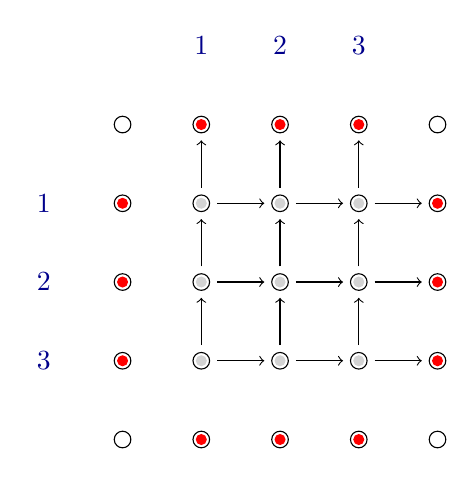
\begin{tikzpicture}
    % labels
    \path[darkblue] (1,5) node{1} (-1,1) node{3};
    \path[darkblue] (2,5) node{2} (-1,2) node{2};
    \path[darkblue] (3,5) node{3} (-1,3) node{1};
    % loop over the lattice points
    \foreach \i in {0,...,4}
      \foreach \j in {0,...,4}{
        \draw (\i,\j) circle(3pt);
        % check if (\i,\j) > (2,2)
        \ifnum \i = 0
          \ifnum \j = 1 
            \fill[red] (\i,\j) circle(2pt);
          \fi
          \ifnum \j = 2 
            \fill[red] (\i,\j) circle(2pt);
          \fi
          \ifnum \j = 3 
            \fill[red] (\i,\j) circle(2pt);
          \fi
        \fi
        \ifnum \i = 1
          \ifnum \j = 1 
            \fill[grey] (\i,\j) circle(2pt);
          \fi
          \ifnum \j = 2 
            \fill[grey] (\i,\j) circle(2pt);
          \fi
          \ifnum \j = 3 
            \fill[grey] (\i,\j) circle(2pt);
          \fi
        \fi
        \ifnum \i = 2
          \ifnum \j = 1 
            \fill[grey] (\i,\j) circle(2pt);
          \fi
          \ifnum \j = 2 
            \fill[grey] (\i,\j) circle(2pt);
          \fi
          \ifnum \j = 3 
            \fill[grey] (\i,\j) circle(2pt);
          \fi
        \fi
        \ifnum \i = 3
          \ifnum \j = 1 
            \fill[grey] (\i,\j) circle(2pt);
          \fi
          \ifnum \j = 2 
            \fill[grey] (\i,\j) circle(2pt);
          \fi
          \ifnum \j = 3 
            \fill[grey] (\i,\j) circle(2pt);
          \fi
        \fi
        \ifnum \i = 4
          \ifnum \j = 1 
            \fill[red] (\i,\j) circle(2pt);
          \fi
          \ifnum \j = 2 
            \fill[red] (\i,\j) circle(2pt);
          \fi
          \ifnum \j = 3 
            \fill[red] (\i,\j) circle(2pt);
          \fi
        \fi
        \ifnum \j = 0
          \ifnum \i = 1 
            \fill[red] (\i,\j) circle(2pt);
          \fi
          \ifnum \i = 2 
            \fill[red] (\i,\j) circle(2pt);
          \fi
          \ifnum \i = 3 
            \fill[red] (\i,\j) circle(2pt);
          \fi
        \fi
        \ifnum \j = 4
          \ifnum \i = 1 
            \fill[red] (\i,\j) circle(2pt);
          \fi
          \ifnum \i = 2 
            \fill[red] (\i,\j) circle(2pt);
          \fi
          \ifnum \i = 3 
            \fill[red] (\i,\j) circle(2pt);
          \fi
        \fi
      };
    %Vertical arrows
    \draw [->] (1,1.2) -- (1,1.8);
    \draw [->] (1,2.2) -- (1,2.8);
    \draw [->] (1,3.2) -- (1,3.8);
    \draw [->] (2,1.2) -- (2,1.8);
    \draw [->] (2,2.2) -- (2,2.8);
    \draw [->] (2,3.2) -- (2,3.8);
    \draw [->] (3,1.2) -- (3,1.8);
    \draw [->] (3,2.2) -- (3,2.8);
    \draw [->] (3,3.2) -- (3,3.8);
    
    %Horizontal arrows
    \draw [->] (1.2,1) -- (1.8,1);
    \draw [->] (2.2,1) -- (2.8,1);
    \draw [->] (3.2,1) -- (3.8,1);
    \draw [->] (1.2,2) -- (1.8,2);
    \draw [->] (2.2,2) -- (2.8,2);
    \draw [->] (3.2,2) -- (3.8,2);
    \draw [->] (1.2,3) -- (1.8,3);
    \draw [->] (2.2,3) -- (2.8,3);
    \draw [->] (3.2,3) -- (3.8,3);
  \end{tikzpicture}
\end{center}
This makes the implementation of the energy really compact. The magnetization of the lattice is still given by Eguation (\ref{eq:Magnetization}), and we can implement the energy and magnetization of a two dimensional lattice by the code below.
\begin{lstlisting}
for(i from 1 to L+1)
        for(j from 1 to L+1)
            E -= R(i,j)*R(i,j+1) + R(i,j)*R(i-1,j)
            M += R(i,j)
\end{lstlisting}
You might wonder why we need the extra row below and the column on the left hand side of the lattice, they are not in use when calculating the values of a lattice, but when we begin to study the time evolution they are essential.\par
We have seen that $\Delta E$ is the energy difference between two dependent microstates (the difference is only one flip), but since the energy of the new microstate only depends on the energy of the previous microstate, the flipped spin and its neighbours, we can compute this energy by finding the energy contributed by the old spin and replace it with the energy contributed by the new spin. Mathematically the same idea can be derived by this:
\begin{equation*}
\Delta E=E_{new}-E_{late}=-J\sum_{<kl>}^Ns_{k,2}s_{l,2}+J\sum_{<kl>}^Ns_{k,1}s_{l,1}= J\sum_{<kl>}^Ns_k(s_{l,1}-s_{l,2})
\end{equation*}
where the index 1 is used for the late states and 2 is used for the new. In the deriving above one need to use that the neighbours are unchanged during the flip ($s_{k,1}=s_{k,2}-s_k$), and further one need to use that $s_{l,1}-s_{l,2}=s_{l,1}$, which is easy to show using $s_{l,1}\pm1$ and $s_{l,2}\mp1$. Finally we get the expression we are looking for
\begin{equation}
\Delta E=2Js_{l,1}\sum_{<k>}^4s_k.
\end{equation}
For the magnetization the approach is really similar
\begin{equation}
\Delta M=M_2-M_1=\sum_{<k>}^Ns_{k,2}-\sum_{<k>}^Ns_{k,1}=-2s_{k,1}
\end{equation}
This makes the differences easy to implement, but we need to keep all the added boundaries in case the flipped spin is on the left or lower rand. If we assume that we have a $L+2\times L+2$ lattice like implemented in the previous subsection, one can implement this like shown below
\begin{lstlisting}
E_late  = -(R_late*R(i+1,j) + R_late*R(i,j+1) + R_late*R(i+2,j+1) + R_late*R(i+1,j+2))
E_new   = -(R(i+1,j+1)*R(i+1,j) + R(i+1,j+1)*R(i,j+1) + R(i+1,j+1)*R(i+2,j+1) + R(i+1,j+1)*R(i+1,j+2))
Delta_E = E_new - E_late
Delta_M = -2*R_late
\end{lstlisting}
where we have been flipping the spin with indices (j+1,i+1) and $R_{late}$ was the spin value before we did the flip.

\subsection{The Metropolis algorithm}
The indices of the spin which is going to be flipped are withdrawn randomly from the RNG, which determines the energy difference, which again elects if the flip is accepted or not. The Metropolis method used in this project is closely linked to Boltzmann's distribution, and will discard all flips which mismatches with the distribution. This is done by computing the ratio of the acceptance probabilities 
\begin{equation}
\frac{A_{j\rightarrow i}}{A_{i\rightarrow j}}=e^{-(E_i-E_j)\beta}=e^{-\Delta E\beta}
\end{equation}
where $A_{j\rightarrow i}$ is the conditional probability to accept the new state ($i$). If this ratio is greater or equal to 1, the flip is always accepted, otherwise a random number is withdrawn and compared to $e^{-\Delta E\beta}$. The specific Metropolis algorithm used in this project goes like
\begin{equation}
\text{Flip} =
    \begin{cases}
            \text{if } e^{-\Delta E\beta}\geq1,\Rightarrow \quad \text{Accept}\\
            \text{if } e^{-\Delta E\beta}<1,\Rightarrow
            \begin{cases}
            		\text{if } r\geq e^{-\Delta E\beta},\Rightarrow & \text{Accept}\\
            		\text{if } r<e^{-\Delta E\beta},\Rightarrow & \text{Discard}
            \end{cases}
    \end{cases}
\end{equation}
where $r$ is the random number mentioned above. The implementation is really straight forward with several if-statements, but one must remember to save the energy and flip from the previous microstate in case the flip is discarded. 

\subsection{Minimize CPU time}
We want to run the program for a large number of Monte Carlo cycles, and this will take time. To make this time as short as possible, we need to remove all unnecessary things. This could be done manually, but a better choice is to use a optimization flag which does this perfectly. We have used the flag called \textit{gcc}, and in practice this is done by pasting a snippet into the pro file. \par\vspace{5mm}

Another important thing to do before running the program for millions of Monte Carlo cycles is to parallelize the code to let one part of the processor work with one parameter separately from the others. This lets us use all the processor cores and we exploit the power of the computer in the best way.  
We decided to use MPI because it's easy to implement i QTcreator. First we need to specify the number of processes we want to run, which is done by choosing the folder where MPI is saved and writing a short code in the run menu. I guess the exact implementation isn't that important, it can be found in the github repository \cite{Repository}.\par\vspace{5mm}

Furthermore we need to use data types that can handle large numbers. Some numbers are going to be very large, and to avoid overflow, these have to be declared as long ints and doubles instead of ints and floats respectively.

\section{Results}
\subsection{Average energy and magnetization}
We have been study how the average values of the energy and the magnetization varying as function of the number of flips for both an ordered and a random initial lattice and for a couple of temperatures ($T'=1.0$ and $T'=2.4$). We use a system with $L=20$ spins in each direction and flip $10^8$ times. The plots are found in Figure (\ref{4c_random}) and (\ref{4c_ordered}). 
\begin{figure}[H]
\centering
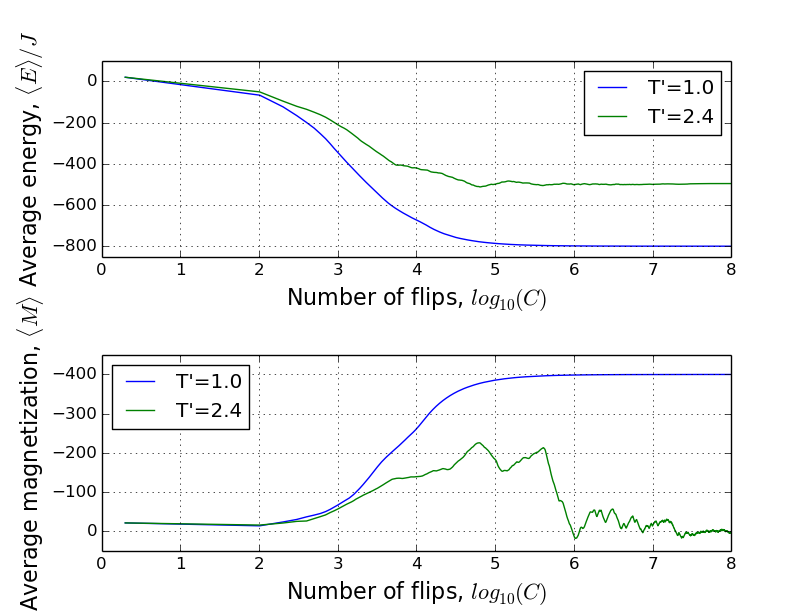
\includegraphics[width=150mm]{plot_4c_E_M_random_new.png}
\caption{Average energy and magnetization for $T'=1.0$ and $T'=2.4$ when we start with a random lattice. Notice: The average magnetization is not the absolute value as it's supposed to be. \label{4c_random}}
\end{figure}
\begin{figure}[H]
\centering
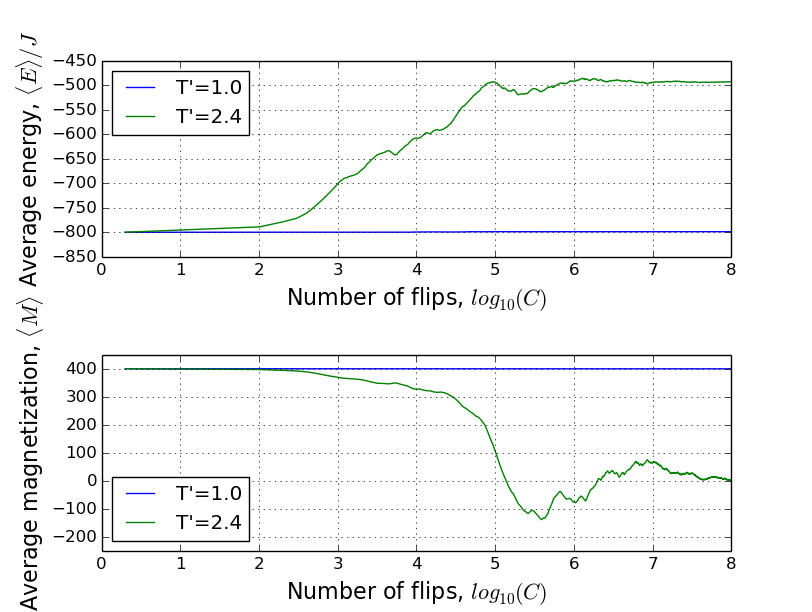
\includegraphics[width=150mm]{plot_4c_E_M_ordered_new.png}
\caption{Average energy and magnetization for $T'=1.0$ and $T'=2.4$ when we start with an ordered lattice. Notice: The average magnetization is not the absolute value as it's supposed to be. \label{4c_ordered}}
\end{figure}
When we start with a random lattice and the temperature is $T'=1.0$, we can see that the average energy and magnetization stabilizes after we have been doing $\sim 10^7$ flips, and for the ordered beginning lattice case the average values are stable from the start. For $T'=2.4$ the situation is quite different; the average values of all the quantities are pretty unstable except for the average energy of the random lattice, which stabilizes after a time. 

\subsection{Ratio of accepted flips and total flips}
We have also been studying the behaviour of the number of accepted flips as function of total number of spins for a lattice of size $L=20$ and in total $10^8$ flips. The result can be found in Figure (\ref{4c_accept}), where we have been experimented with a couple of temperatures ($T'=1.0$ and $T'=2.4$) where we both start with an ordered and a random matrix. The plots are normalized such that we plot the ratio of accepted flips and flips in total (probability for accepting a flip) on the y-axis and the numbers of flips on the x-axis.  
\begin{figure}[H]
\centering
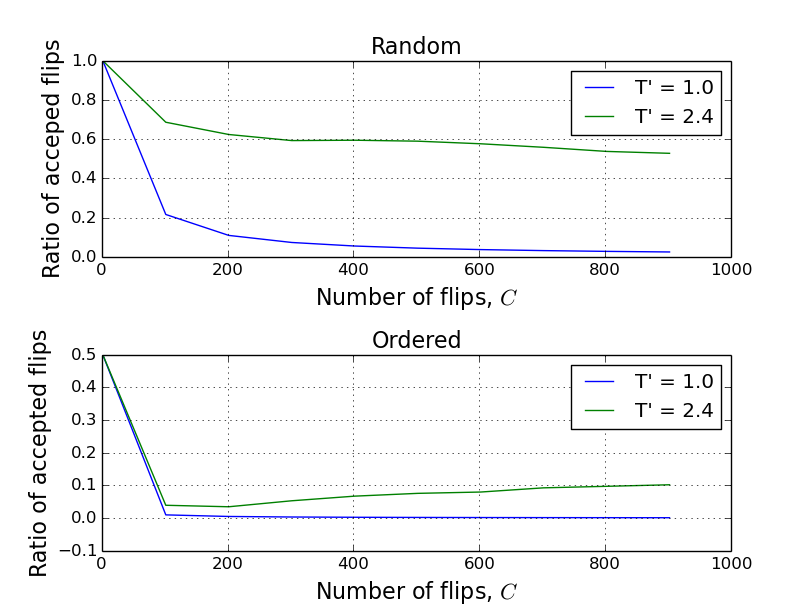
\includegraphics[width=150mm]{accept_vs_MCc_newnew.png}
\caption{The ratio of accepted flips and the total number of flips. The upper subplot shows how the behaviour is when we start with a random lattice with the temperatures $T'=1.0$ and $T'=2.4$, while the lower shows how the behaviour is when the initial lattice is ordered. \label{4c_accept}}
\end{figure}
As we can see the ratio stabilizes for $T'=1.0$ for both of the initial lattices, while it's still unstable for $T'=2.4$ in both cases. 

\subsection{Probability and energy variance}
We want to compute the probability of finding the system in different energy states after it has reached steady state for both of the temperatures studied above ($T'=1.0$ and $T'=2.4$). Again we use a system of size $L=20$ and run for $10^6$ configurations. The results for $T'=1.0$ and $T'=2.4$ are plotted in histograms which can be found in Figure (\ref{4c_prob_t=1}) and (\ref{4c_prob_t=2.4}) respectively. 
\begin{figure}[h]
\centering
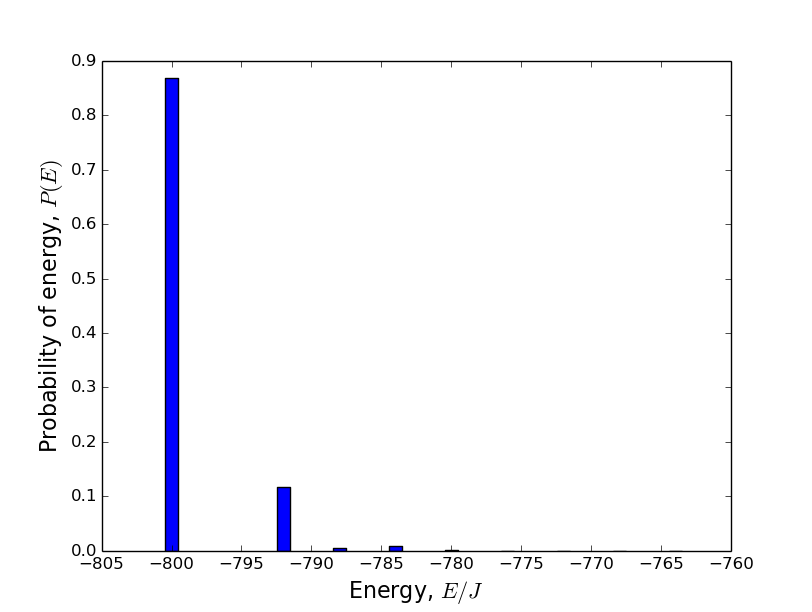
\includegraphics[width=120mm]{plot_4d_prob_T=1_0_N=1e6.png}
\caption{The probability of finding the system in the possible energy states for $T'=1.0$.\label{4c_prob_t=1}}
\end{figure}
\begin{figure}[h]
\centering
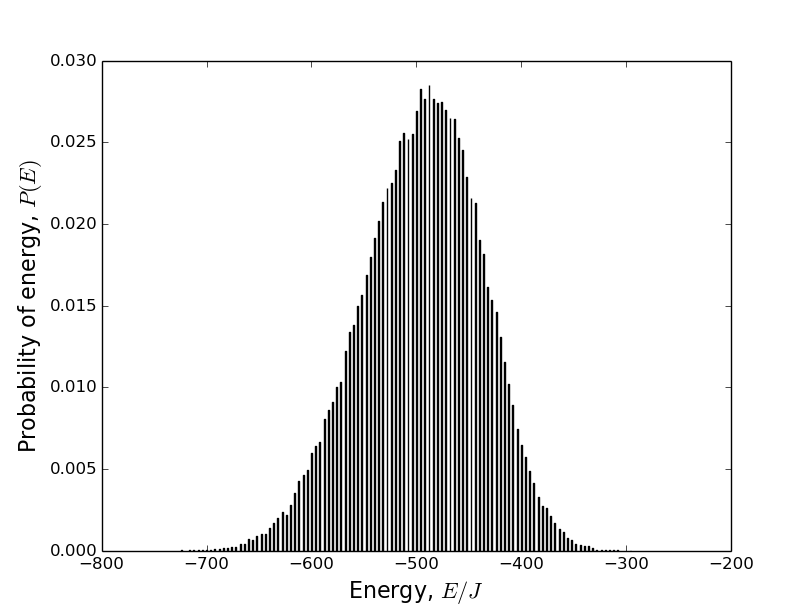
\includegraphics[width=120mm]{plot_4d_prob_T=2_4_N=1e6.png}
\caption{The probability of finding the system in the possible energy states for $T'=2.4$ \label{4c_prob_t=2.4}}
\end{figure}
\newline We can see that the fluctuations are small for $T'=1.0$, most of the time the energy of the system is $E/J=-800$, sometimes the energy is $E/J=-792$ and for a some short moments the energy is lower than this. For $T'=2.4$ the situation is really different, we get a lot of possible energy states and the energy seems to be distributed like a skew normal distribution between them with the maxima at $E/J\approx -510$. I will define the equilibrium as the case when the system fluctuates around the steady state.\par\vspace{5mm}

The energy variance of the system when $T'=1.0$ is estimated by the computer to be $\sigma_E^2/J^2=16.1344$, which correspond to a standard deviation of $\sigma_E/J=4,0168$. When $T'=2.4$ we have a energy variance of $\sigma_E^2/J^2=3194.79$, which is in fact much larger than when the temperature was $T'=1.0$!

\subsection{The behaviour of systems around the critical temperature}
An interesting study is how the system changes for different temperatures and system sizes. We have been looking at systems of size $L=40, 60, 80$ and $100$, and studied how the average energy, average absolute magnetization, heat capacity and susceptibility behave around the critical temperature (from the theory we know that $T_c'\approx2.269$). In Figure (\ref{4e_E}) one can find how the average energy changes in the interval $T'\in[2.200,2.310]$. The graphs are normalized so that we can compare the different system sizes effortlessly. 
\begin{figure}[h]
\centering
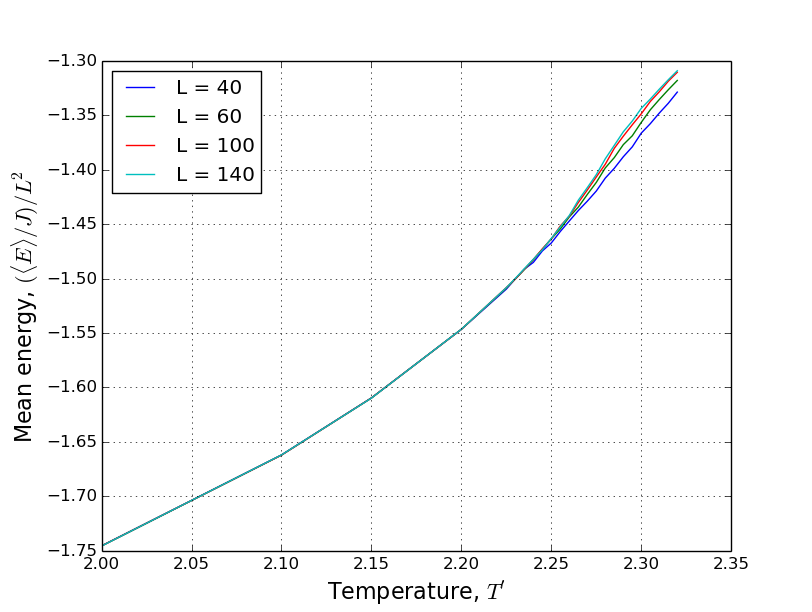
\includegraphics[width=110mm]{plot_4e_E.png}
\caption{The average energy as function of dimensionless time $T'$ around the expected critical temperature ($T'\in[2.200,2.310]$) for various system sizes. \label{4e_E}}
\end{figure}
We can see that the energies follow each other to a point where we get a spread, and all the graphs are strictly increasing in all the interval. The plot of the average absolute magnetization is found in Figure (\ref{4e_M}), where we still are using the interval $T'\in[2.200,2.310]$ and normalized graphs.
\begin{figure}[H]
\centering
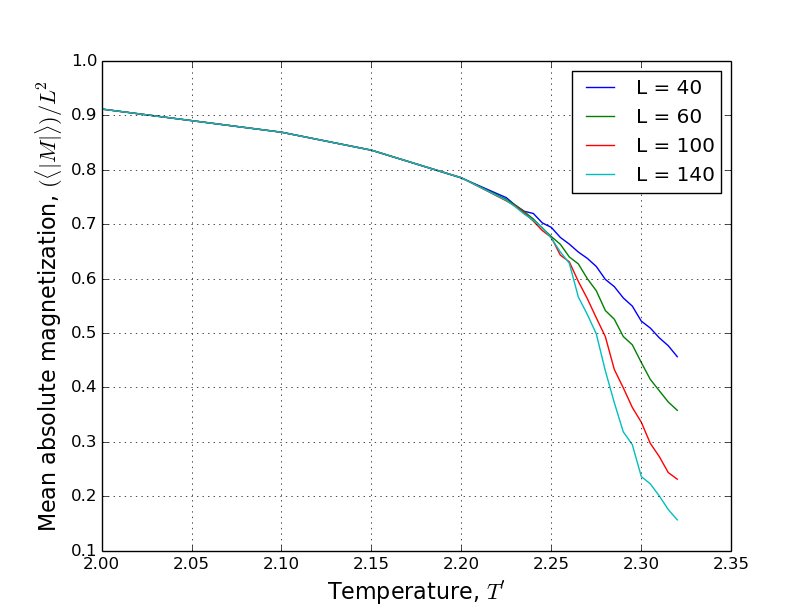
\includegraphics[width=110mm]{plot_4e_M.png}
\caption{The average absolute magnetization as function of dimensionless time $T'$ around the expected critical temperature ($T'\in[2.200,2.310]$) for various system sizes. \label{4e_M}}
\end{figure}
In the same way as for the average energy the average absolute magnetization get a spread at a point, but they are now strictly \textit{decreasing}. We observe that the larger the system is, the faster the graph subsides. Further the heat capacity plot is presented in Figure (\ref{4e_heat}), with $T'\in[2.200,2.310]$ and normalized graphs.
\begin{figure}[H]
\centering
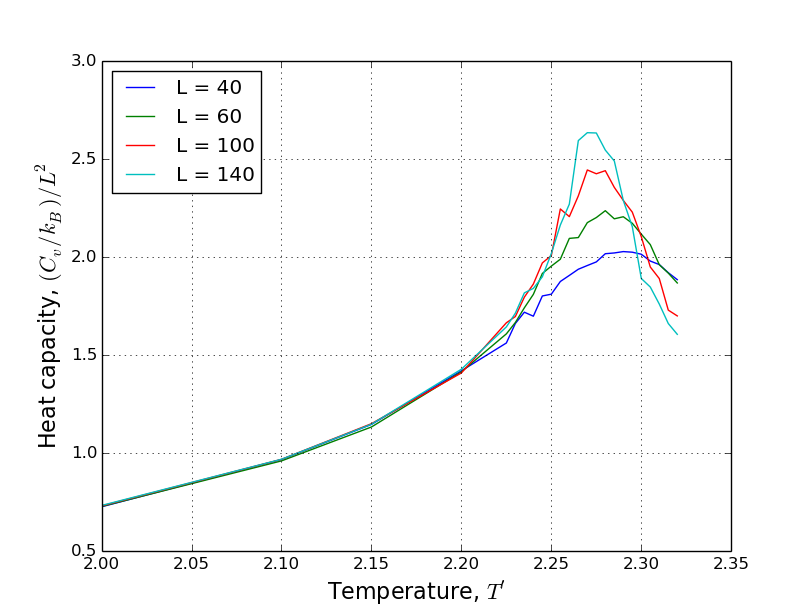
\includegraphics[width=110mm]{plot_4e_heat.png}
\caption{The heat capacity as function of dimensionless time $T'$ around the expected critical temperature ($T'\in[2.200,2.310]$) for various system sizes. \label{4e_heat}}
\end{figure}
This is a really exciting plot since we have situations where the temperatures are increasing but the heat capacities are still decreasing! From the graphs we can read that the maximums for $L=40$, $L=60$, $L=100$ and $L=140$ are $T'=2.292$, $T'=2.283$, $T'=2.277$ and $T'=2.273$ respectively, so the maxima are moding to the left when the system size is increasing. Finally we have plotted the susceptibility as function of the dimensionless temperature $T'$ around the expected critical temperature with normalized graphs for the four system sizes. The plot is found in Figure (\ref{4e_X}).
\begin{figure}[H]
\centering
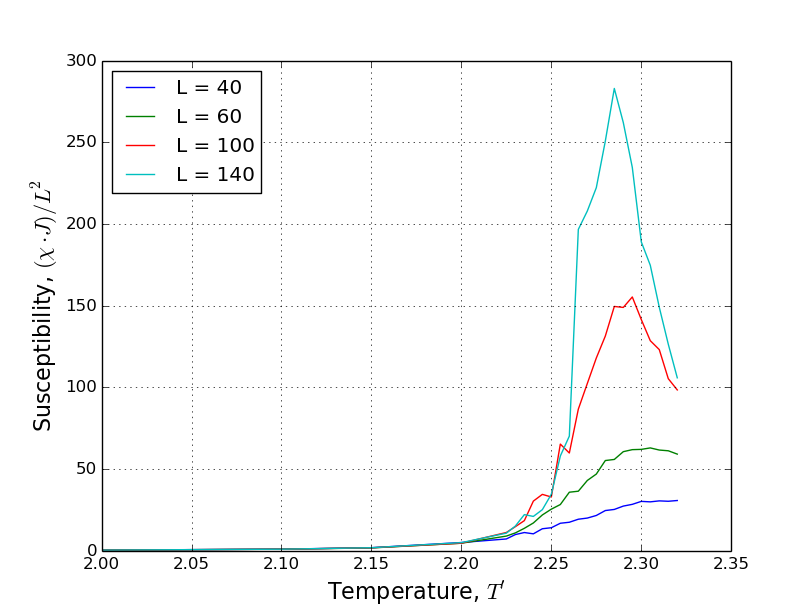
\includegraphics[width=110mm]{plot_4e_X.png}
\caption{The susceptibility as function of dimensionless time $T'$ around the expected critical temperature ($T'\in[2.200,2.310]$) for various system sizes. \label{4e_X}}
\end{figure}
In the same manner as for the heat capacity we can see that the susceptibility after a point is decreasing for increasing temperatures. For $L=40$, $L=60$, $L=100$ and $L=140$ the maximum points are found at $T'=2.317$, $T'=2.303$, $T'=2.293$ and $T'=2.285$ respectively. 

\subsection{Estimation of the critical temperature}
The critical temperature is where the heat capacity and susceptibility have their maximum points, and we have already estimated them in sub section 4.4. The results are clearly represented in Table (\ref{tab:tc}).
\begin{table}[h]
\centering
\caption{The critical temperatures for $L=40$, 60, 100 and 140 read from the heat capacity and susceptibility graphs.}
\label{tab:tc} 
\begin{tabularx}{\textwidth}{XlcrX}
&&\\
\toprule
\multicolumn{3}{c}{Critical temperature $T_c'$}\\
\cline{2-3}
Size, $L$  & heat capacity  & susceptibility\\
\midrule
40   & 2.290  & 2.317\\
60   & 2.283  & 2.303\\
100  & 2.275  & 2.293\\
140  & 2.272  & 2.285\\
\bottomrule
\end{tabularx}
\end{table}
As we can see the critical temperature is decreasing for larger systems. We need to estimate the constant $a$ before we can compute $T_c(L=\infty)$, something I will do with the critical temperatures from the heat capacity. This is done by Equation (\ref{eq:a}), and we can do it for six different combinations of $L$ presented in Table (\ref{tab:as}). 
\begin{table}[H]
\centering
\caption{Estimates of $a$ for different combinations of $L$'s using Equation (\ref{eq:a}) and the data presented in Table (\ref{tab:tc}).}
\label{tab:as} 
\begin{tabularx}{\textwidth}{XXr}
&&\\
\toprule
$L_1$ & $L_2$  & $a$\\
\midrule
40   & 60   & 0.840\\
40   & 100  & 1.000\\
40   & 140  & 1.008\\
60   & 100  & 1.200\\
60   & 140  & 1.155\\
100  & 140  & 1.050\\
\midrule
Average:&& 1.042\\
\bottomrule
\end{tabularx}
\end{table}
We will use the average value to estimate the critical temperature of a system with infinite magnetic moment using Equation (\ref{eq:critical}). Again we can do this in several ways (exact four ways), which are presented in Table (\ref{tab:tcs}).
\begin{table}[H]
\centering
\caption{The critical temperature estimated using Equation (\ref{eq:critical}) and the average estimate of $a$ for all the system sizes $L=40$, 60, 100 and 140.}
\label{tab:tcs} 
\begin{tabularx}{\textwidth}{XlcrX}
&&\\
\toprule
$L$ && $T_c'(L=\infty)$\\
\midrule
40    && 2.265\\
60    && 2.265\\
100   && 2.266\\
140   && 2.264\\
\midrule
Average:&& 2.265\\
\bottomrule
\end{tabularx}
\end{table}
From our measurements we can estimate the critical temperature for a system of infinite magnetic moment to be 
\begin{equation}
T_c'(L=\infty)\approx2.265.
\end{equation}

\subsection{Benchmarks}
Something that is important when doing numerical computations is to compare the results to analytical values. In the theory part we calculated several expectation values of the $2\times2$ lattice analytically, and by running the program for various $C$'s we can compare the numerical result with the analytical. The results are found i Table (\ref{tab:benchmark1}), (\ref{tab:benchmark2}), (\ref{tab:benchmark3}) and (\ref{tab:benchmark4}).
\begin{table}[H]
\centering
\caption{The numerical values compared to the exact analytical value for various numbers of flips ($C\in[10^2,10^9]$) for the average energy of the case when $L=2$.}
\label{tab:benchmark1} 
\begin{tabularx}{\textwidth}{XlXrXrXrXrX}
&&&&\\
\toprule
\multicolumn{5}{c}{Average energy $\langle E\rangle/J$}\\
\cline{2-3}
Total flips  & Analytical  & Numerical && Absolute error\\
\midrule
1e2   & -7.98393  & -5.94059   && 2.04334e-00\\
1e3   & -7.98393  & -7.79221   && 1.9172e-01\\
1e4   & -7.98393  & -7.95520   && 2.873e-02\\
1e5   & -7.98393  & -7.98600   && 2.07e-03\\
1e6   & -7.98393  & -7.98445   && 5.2e-04\\
1e7 	  & -7.98393  & -7.98377   && 1.6e-04\\
1e8   & -7.98393  & -7.98401   && 8e-05\\
1e9   & -7.98393  & -7.98385   && 8e-05\\
\bottomrule
\end{tabularx}
\end{table}
\begin{table}[H]
\centering
\caption{The numerical values compared to the exact analytical value for various numbers of flips ($C\in[10^2,10^9]$) for the average absolute magnetization of the case when $L=2$.}
\label{tab:benchmark2} 
\begin{tabularx}{\textwidth}{XlXrXrXrXrX}
&&&&\\
\toprule
\multicolumn{5}{c}{Average absolute magnetization $\langle |M|\rangle$}\\
\cline{2-3}
Total flips  & Analytical  & Numerical && Absolute error\\
\midrule
1e2 & 3.99464  & 3.26733  && 7.2731e-01\\
1e3 & 3.99464  & 3.92607  && 6.857e-02\\
1e4 & 3.99464  & 3.98460  && 1.004e-02\\
1e5 & 3.99464  & 3.99530  && 6.6e-04\\
1e6 & 3.99464  & 3.99490  && 2.6e-04\\
1e7 & 3.99464  & 3.99456  && 8e-05\\
1e8 & 3.99464  & 3.99459  && 5e-05\\
1e9 & 3.99464  & 3.99462  && 2e-05\\
\bottomrule
\end{tabularx}
\end{table}
\begin{table}[H]
\centering
\caption{The numerical values compared to the exact analytical value for various numbers of flips ($C\in[10^2,10^9]$) for the heat capacity of the case when $L=2$.}
\label{tab:benchmark3} 
\begin{tabularx}{\textwidth}{XlXrXrXrXrX}
&&&&\\
\toprule
\multicolumn{5}{c}{Heat capacity $C_v/k_B$}\\
\cline{2-3}
Total flips  & Analytical  & Numerical && Absolute error\\
\midrule
1e2   & 0.128329  & 12.2341   && 1.2105771e+01\\
1e3   & 0.128329  & 1.61916   && 1.490831e-00\\
1e4   & 0.128329  & 0.356358  && 2.28029e-01\\
1e5   & 0.128329  & 0.111803  && 1.6526e-02\\
1e6   & 0.128329  & 0.124174  && 4.155e-03\\
1e7 	  & 0.128329  & 0.129631  && 1.302e-03\\
1e8   & 0.128329  & 0.127682  && 6.47e-04\\
1e9   & 0.128329  & 0.128920  && 5.91e-04\\
\bottomrule
\end{tabularx}
\end{table}
\begin{table}[H]
\centering
\caption{The numerical values compared to the exact analytical value for various numbers of flips ($C\in[10^2,10^9]$) for the susceptibility of the case when $L=2$.}
\label{tab:benchmark4} 
\begin{tabularx}{\textwidth}{XlXrXrXrXrX}
&&&&\\
\toprule
\multicolumn{5}{c}{Susceptibility $\chi\cdot J$}\\
\cline{2-3}
Total flips  & Analytical  & Numerical && Absolute error\\
\midrule
1e2   & 15.9732  & 3.21537   && 1.27578e+01\\
1e3   & 15.9732  & 0.406387  && 1.55668e+01\\
1e4   & 15.9732  & 13.1151   && 2.8581e-00\\
1e5   & 15.9732  & 15.8714   && 1.018e-01\\
1e6   & 15.9732  & 15.9627   && 1.05e-02\\
1e7 	  & 15.9732  & 15.9622   && 1.1e-02\\
1e8   & 15.9732  & 15.9706   && 2.6e-03\\
1e9   & 15.9732  & 15.9731   && 1e-04 \\
\bottomrule
\end{tabularx}
\end{table}
The tendency is that the error decreases as we increase the number of flips. In Figure(\ref{error}) the absolute error is plotted for all the quantities above.

\begin{figure}[H]
\centering
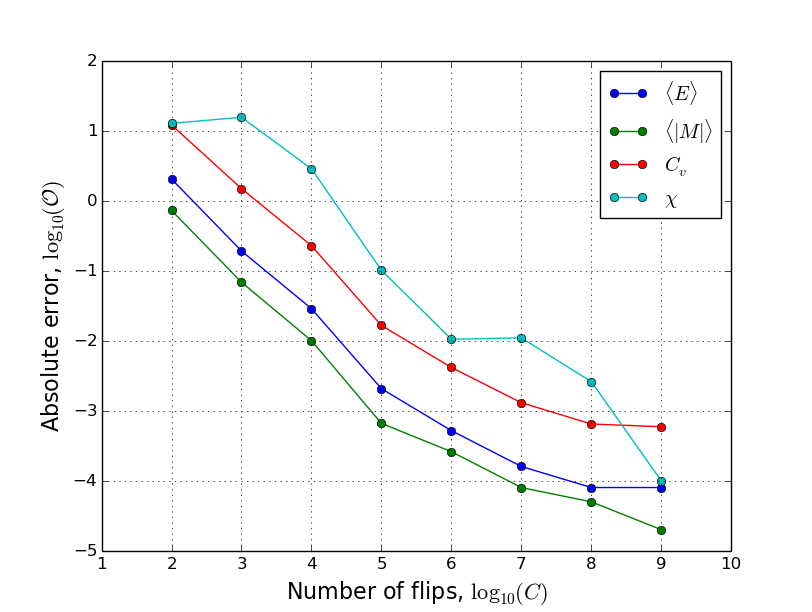
\includegraphics[width=120mm]{error_plot.png}
\caption{Absolute error plotted as a function of the number of flips with logaritmic axis for the average energy, the average magnetization, heat capacity and susceptibility.\label{error}}
\end{figure}

\subsection{Time analyses with and without parallelizing}
To study the CPU time we ran the program for $L=2$ and in total $C=10^8$ before and after implementing the parallelizing, and used $n=10$ processes. A total number of $10^8$ flips then corresponds to $C=10^7$ for each process, and we got the results presented in Table (\ref{tab:timeParallelize}). 
\begin{table}[H]
\centering
\caption{With parallelization for $C=10^8$ flips and without parallelization for $n=10$ processes and $C=10^7$ flips (in total $10^8$ flips).}
\label{tab:timeParallelize} 
\begin{tabularx}{\textwidth}{XlcXrX}
&&\\
\toprule
\multicolumn{3}{c}{Total time [s]}\\
\cline{2-3}
Running  & With parallelization  & Without parallelization \\
\midrule
1	& 13.32  & 30.36    \\
2   & 13.72  & 30.09    \\
3   & 14.76  & 30.35    \\
4   & 13.62  & 30.44    \\
5   & 13.59  & 30.29    \\
6 	& 13.21  & 30.54    \\
7 	& 14.05  & 29.98    \\
8   & 13.80  & 30.05    \\
9   & 14.01  & 30.48    \\
10  & 13.66  & 32.13    \\
\midrule
Average: & 13.78 & 30.47 \\
\bottomrule
\end{tabularx}
\end{table}
We observe that the program uses more than twice as long time without parallelization compared with when it is parallelized. 

\section{Discussion}
In the Result section we found the average energy and magnetization to be stable after a short time for $T'=1.0$, but not for $T'=2.4$, which makes sense because we get more energy and fluctuations for higher temperatures. For $T'=1.0$ the system converges to an energy near $\langle E\rangle/J=-800$, which is the situation when all the spins point in the same direction. From the probability distribution of the energy when $T'=1.0$ (see Figure (\ref{4c_prob_t=1})) one can see that after the equilibrium is reached, we will have energies close to $\langle E\rangle/J=-800$ most of the time, so these results match. When all the spins are pointing in the same direction we will in general have an average magnetization of $\pm L^2$. On the other hand we can see that the system converges to an average energy of $\langle E\rangle/J\approx-510$ when we deal with a temperature of $T'=2.4$, and this is reasonable because we have higher energies for higher temperatures. If we compare this to the probability distribution of the same temperature found in Figure (\ref{4c_prob_t=2.4}), we can see that the most likely state is when $\langle E\rangle/J\approx-510$, but there is more fluctuation in the system than for $T'=1.0$. The average magnetization seems to converge against $\langle M\rangle=0$, which is what we expect from the theory.\par\vspace{5mm}

The average energies and magnetizations converge against the same steady state no matter if we start with a ordered or random lattice, but a main difference is how long time the system needs to reach equilibrium. If we choose a ordered lattice of $T'=1.0$, we can see that the system is in equilibrium from the beginning. Anyway we can with certainty state that we are in equilibrium after $10^7$ flips for $T'=1.0$, and perhaps some longer for $T'=2.4$ (this system will fluctuate about the steady state).\par\vspace{5mm}

We found the variance to increase a lot when we increased the temperature from $T'=1.0$ to $T'=2.4$, something that happens because of the spreading of possible energies for $T'=2.4$. The variance of $T'=1.0$ was computed to be $\sigma_E^2\approx16$, which gives a standard deviation of $\sim 4$, which again corresponds to $68\%$ of the energy being in the interval $E\in[-792,-800]$, which is reasonable. \par\vspace{5mm}

When it comes to the number of accepted configurations we found this stabilizing near 0 after a time for $T'=1.0$. This happens because we are close to the equilibrium, which means that the Metropolis algorithm is discarding almost all of the flips. For the ordered lattice we can see that equilibrium is reached after $\sim200$ flips, which is small but logical because an ordered lattice is close to equilibrium. For a random lattice it takes some longer to reach equilibrium, because we probably are far from equilibrium. For $T'=2.4$ we cannot determine what the ratio corresponds to for sure, nor we can say anything about the time used to reach equilibrium. We should have studied the behaviour for a longer time. \par\vspace{5mm}

The normalized average energy and absolute magnetization around the critical temperature was much the same for all the system sizes until a point where we got the spread. This happens because we have systems with finite magnetic moments, where the smallest system deviates most from the exact infinite magnetic moment solution and so on.\par\vspace{5mm}

The critical temperature of a system of infinite size was estimated using the maximum points of the heat capacity, which were found reading from the graph. This readout method might generates errors, so we need to look carefully. To minimize these errors, we could have done a polynomial regression of second order around the peaks and found the exact top point of these regression graphs, then we would avoid much of the errors. Furthermore we have seen that there are multiple ways to calculate the constant $a$, and when we got $a$ there are still some ways to calculate the critical temperature. This makes it easy to manipulate the results to be close to the exact critical temperature, but by using the average value we are not so vulnerable. The result was close to the exact solution with a error of $\sim 10^{-3}$.\par\vspace{5mm}

For the benchmarks we got approximately the results we expected. The absolute error decreases when we increase the number of flips, which is a good result. In general we observe that the absolute error of the heat capacity and susceptibility are some larger than the error of the energy and absolute magnetization. The reason for this is that we add the error from $\langle E\rangle$ to the error from $\langle E^2\rangle$ and obtain a poor precision compared to the other quantities. The result is similar for the susceptibility, where we add the errors gotten from $\langle M\rangle$ to the error from $\langle M^2\rangle$. When we are finding the number of flips needed to achieve a good agreement, we need to look at the quantity which generates most errors, which is the susceptibility. After $10^6$ flips we have an error of $\sim10^{-2}$, which should be sufficient.\par\vspace{5mm}

We have seen that the computer is able to run the program with considerably shorter CPU time after parallelization compared with before, and the reason to this is that the parallelization forces all the processor cores to run with maximum effect. We chose to do this study for a $2\times2$ lattice to minimize the time used for setting up the matrix. If we assume that one process only can run on one core, we might could reduce this time further by having the number of processes as an integer multiple the number of cores of the processor. A average computer nowadays has 4 processor cores, so by choosing for instance 8 processes, we could perhaps achieve a better result.

\section{Conclusion}
All in all I am really satisfied with the results of this project. The average plots match the probability histograms and agree with my intuitive understanding. The benchmarks also indicate that our numerical implementation is correct, the absolute error is small and decreases for larger systems like we would expect. We have gotten a critical temperature which is close to the analytical value, and all benchmarks seems to be good. \par\vspace{5mm}

Like in all other projects, there exist improvements. For instance we could have studied the behaviour of the systems for a larger numbers of temperatures in the same interval (smaller $\Delta T'$), so the curves had been smoother. This would make it easier to read the critical temperatures, and maybe we could have estimated the critical temperature $T_c'(L=\infty)$ with even better precision? We could also have done this by regression like discussed in the discussion section. Another thing we could have done is to study the number of accepted flips for longer times, and plotted the average absolute magnetization instead of the absolute magnetization in the first subsection of Results, but these improvements are just visual. We could of course have let the program run for longer times, so estimate the numerical values even better. Anyway I feel happy with the results, and this would not be possible without my great collaborators.\par\vspace{5mm}

I think this project was very interesting and informative, and I like the way it links computational physics with thermal physics. We experienced that smaller temperature steps would be useful when we were studying the behaviour of the systems in exercise 4e, so a suggestion of a smaller $\Delta T'$ would maybe be appropriate? We also think the units of the temperature should have been specified clearer in the project description, because the dimensionless $T$ (which I decided to call $T'$) is the same as the $T$ with dimension temperature. Apart from that I cannot find any improvements, so well done with the problem set!

\section{Bibliography}
\begingroup
\renewcommand{\section}[2]{}
\begin{thebibliography}{}
\bibitem{MHJ15}
  Hjorth-Jensen, Morten.
  Computational Physics, Lecture Notes Fall 2015.
  Department of Physics, University of Oslo.
  August 2015.
\bibitem{Ising}
  Nature - History of the Ising model: 		(November 7th 2016)\newline
  \url{http://www.nature.com/nphys/journal/v11/n12/full/nphys3595.html}
\bibitem{Project_text}
  Project description:  (November 8th 2016)\newline
  \url{https://github.com/CompPhysics/ComputationalPhysics/blob/gh-    pages/doc/Projects/2016/Project4/pdf/Project4.pdf}
\bibitem{Repository}
  Github Repository URL:
  \url{https://github.com/richaraf/Comphys_projects/tree/master/Project_4}
\end{thebibliography}
\endgroup
\end{document}